
\lstinputlisting[language=bash,basicstyle=\small]{python_codes/fieldstone_74/keywords.ascii}

\begin{center}
Code at \url{https://github.com/cedrict/fieldstone/tree/master/python_codes/fieldstone_74}
\end{center}

\par\noindent\rule{\textwidth}{0.4pt}

%%%%%%%%%%%%%%%%%%%%%%%%%%%%%%%%%%%%%%%%%%%%%%%%%%%%%%%%%%%%%%%%%%%%%%%%%%%%%%%%%%%%%%%%%%%%
\index{stopics}{$Q_1^+\times Q_1$}

The benchmark is described fully in Section~\ref{MMM-ss:anconv}. 
The following results have been obtained with $k=4$.
MINI $Q_1^+ \times Q_1$ elements are used with an isoparametric mapping. 

The layout of the points is borrowed from \stone~\ref{f09} which 
showcases $Q_1 \times P_0$ elements. 
Special care should be taken with the placement of the bubble node.  
If placed at 
\[
x_4 = \frac{1}{4}(x_0+x_1+x_2+x_3)
\qquad
y_4 = \frac{1}{4}(y_0+y_1+y_2+y_3)
\]
this yields a pressure field with large oscillations. In order to correct the 
problem, I proceed as follows:
\[
r_4 = \frac{1}{4}(r_0+r_1+r_2+r_3)
\qquad
\theta_4 = \frac{1}{4}(\theta_0+\theta_1+\theta_2+\theta_3)
\]
and then $\vec{r}_4=(x_4,y_4)=(r_4 \cos\theta_4,r_4 \sin\theta_4)$.

\begin{lstlisting}
for iel in range(0,nel):
    r[iconV[4,iel]]=r[iconV[0,iel]]+dr/2
    theta[iconV[4,iel]]=theta[iconV[0,iel]]-dtheta/2
    xV[iconV[4,iel]]=r[iconV[4,iel]]*np.cos(theta[iconV[4,iel]])
    yV[iconV[4,iel]]=r[iconV[4,iel]]*np.sin(theta[iconV[4,iel]])
\end{lstlisting}

\begin{center}
\includegraphics[width=7cm]{python_codes/fieldstone_74/results/Vnodes}
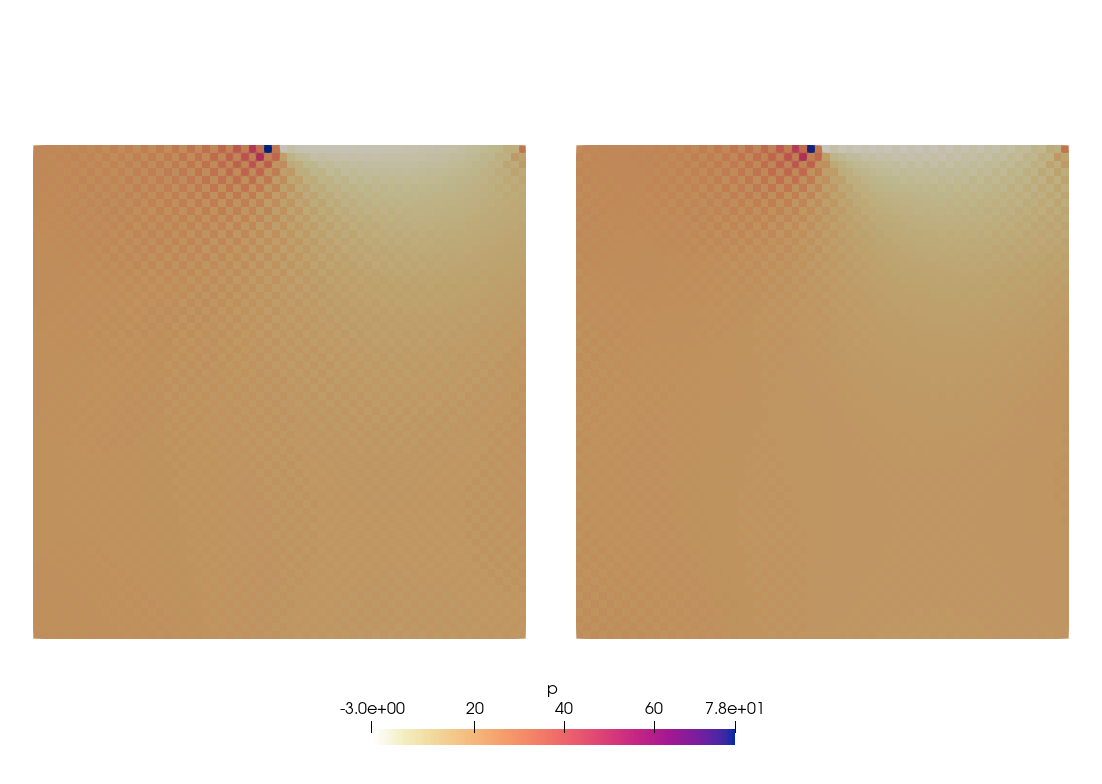
\includegraphics[width=7cm]{python_codes/fieldstone_74/results/pressures}\\
{\captionfont Left: Velocity nodes in the mesh. Right: 
Difference in pressure field when the bubble is placed
at the wrong location (left half of the annulus) and at the right location (right half).}
\end{center}

The pressure nullspace is removed by means of a Lagrange multiplier.

As in \stone~\ref{f21}, I here compute the velocity gradient tensor 
first ${\bm L}(\vec\upnu)=\vec\nabla\vec\upnu$.
I loop over elements. For each element I loop over its velocity nodes and use the $Q_2$ 
shape function derivatives to compute the four components $L_{xx},L_{xy},L_{yx},L_{yy}$ at 
the node and add this value to the node (while keeping track of how many times a value
has been added to the node). In the end I simply compute the average of the values
on each node. From ${\bm L}(\vec\upnu)$ I then compute $\dot{\bm \varepsilon}(\vec\upnu)$. 

We recover a quadratic convergence for the velocity error and a 1.5 index error rate for the 
pressure (which is between the quadratic convergence of the Taylor-Hood element 
and the $Q_1\times P_0$). Note that $h=dr=(R_2-R_1)/nelr=1/nelr$. 

\begin{center}
\includegraphics[width=7cm]{python_codes/fieldstone_74/results/bubble1/errors_v.pdf}
\includegraphics[width=7cm]{python_codes/fieldstone_74/results/bubble2/errors_v.pdf}\\
\includegraphics[width=7cm]{python_codes/fieldstone_74/results/bubble1/errors_p.pdf}
\includegraphics[width=7cm]{python_codes/fieldstone_74/results/bubble2/errors_p.pdf}
\end{center}

%I also computed the error convergence of the strain rate components obtained with 
%the three different methods presented in Section~\ref{ss:nodderiv}
%and we recover a quadratic convergence for methods 2 and 3 while method 1 
%shows an exponent of 1.5:
%\begin{center}
%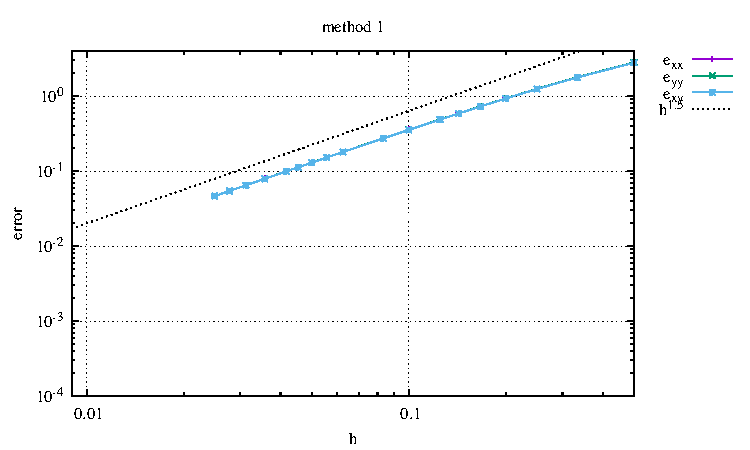
\includegraphics[width=10cm]{python_codes/fieldstone_21/results/errors_sr1.pdf}\\
%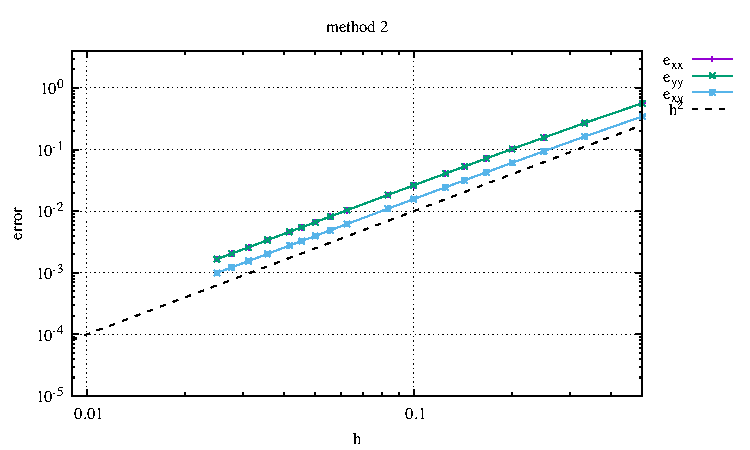
\includegraphics[width=10cm]{python_codes/fieldstone_21/results/errors_sr2.pdf}\\
%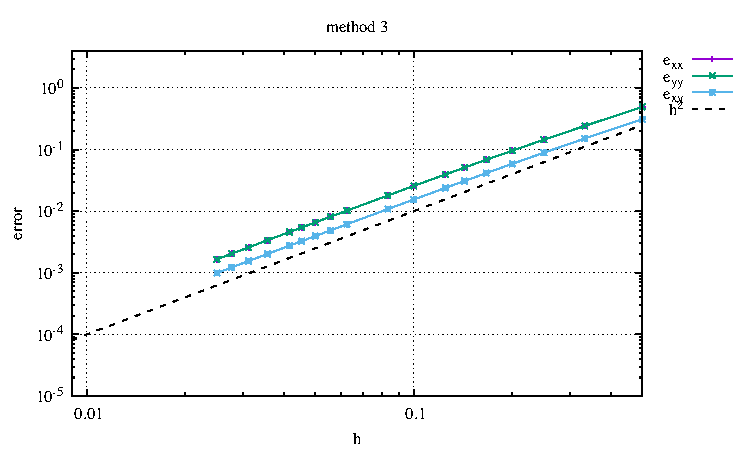
\includegraphics[width=10cm]{python_codes/fieldstone_21/results/errors_sr3.pdf}
%\end{center}

Also the root mean square velocity is logically found to converge to its 
expected analytical value.

\begin{center}
\includegraphics[width=7cm]{python_codes/fieldstone_74/results/bubble1/vrms.pdf}
\includegraphics[width=7cm]{python_codes/fieldstone_74/results/bubble2/vrms.pdf}
\end{center}

This shows that a $3\times 3$ quadrature is to be preferred over a $2\times 2$. 
Higher quadratures do not yield any improvement. 

%The pressure $p$ and its projection onto the $Q_2$ grid at 
%$r=R_1$ and $r=R_2$ are plotted here under:
%\begin{center}
%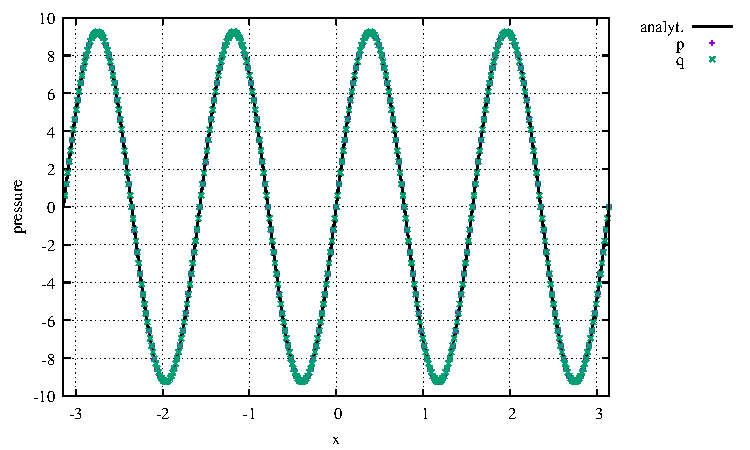
\includegraphics[width=10cm]{python_codes/fieldstone_21/results/pressure_R1.pdf}\\
%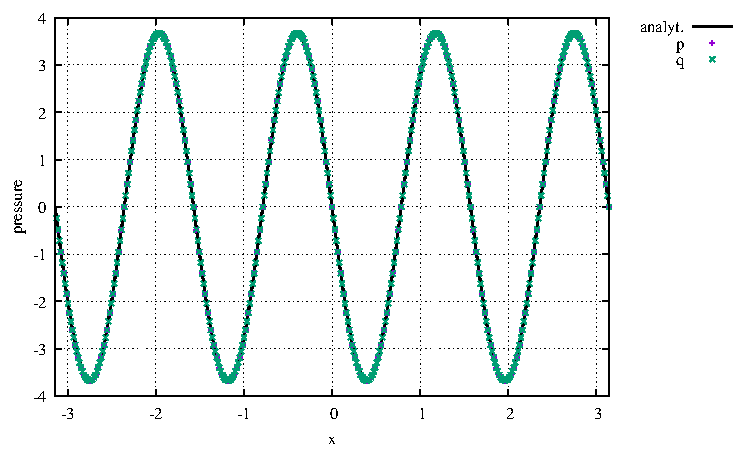
\includegraphics[width=10cm]{python_codes/fieldstone_21/results/pressure_R2.pdf}\\
%{\captionfont Left: pressure $p$ and $q$ at $r=R_1$; Right: 
%pressure $p$ and $q$ at $r=R_2$.}
%\end{center}

\underline{Influence of $\beta$ for bubble 2}:

I fix the quadrature at $3\times 3$ points. 

\begin{center}
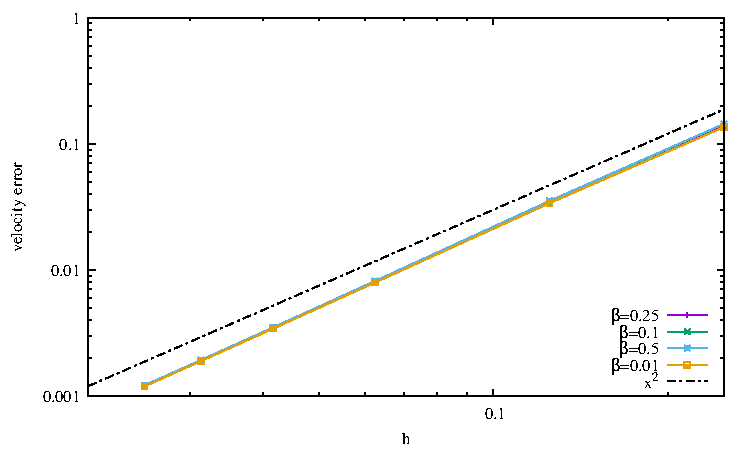
\includegraphics[width=5.5cm]{python_codes/fieldstone_74/results/errors_v}
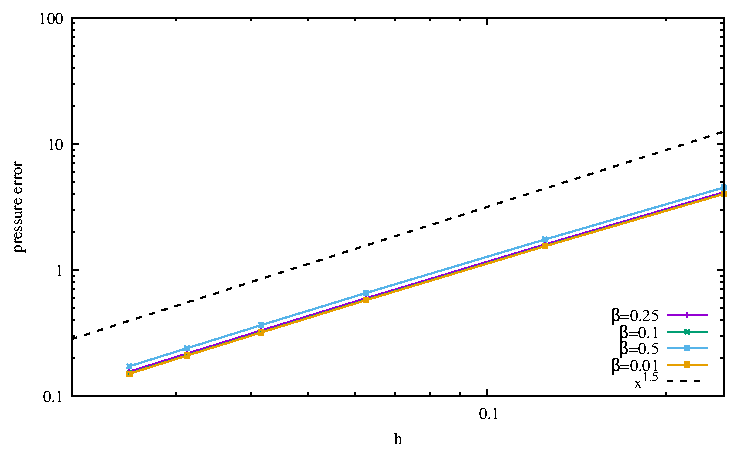
\includegraphics[width=5.5cm]{python_codes/fieldstone_74/results/errors_p}
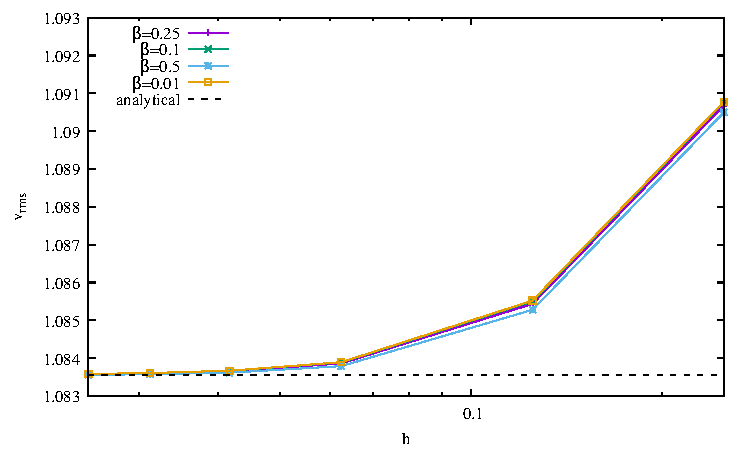
\includegraphics[width=5.5cm]{python_codes/fieldstone_74/results/vrms.pdf}
\end{center}

We see that the value of $\beta$ does not really matter, although 0.5 is probably too large.

